\chapter{On Joining Property Graphs}\label{cha:join}
\epigraph{\textit{A Cypher query walks into a bar and sees two graphs. It walks up to them and says, ``May I join you''?}.}{--- Restating a well known pun on SQL.}

The hight availability of graph data demands for a binary operator combining two distinct graphs into one single graph.
%Since lots of graph data is generated,
% the need of integrating different graphs  becomes more poignant.
Since in the relational model this task is entrusted to join operators, we would expect that similar
tasks already appear to be on graph query languages. As described in Section \ref{sec:informationsintegration}, the join operation is just one of the two operations required for data integration alongside with grouping. While the graph grouping operation has already been defined \cite{JunghannsPR17}, this graph operation is still missing on current \textsc{Graph DataBase Management Systems} (GDBMS).

Despite the term ``join'' appearing in graph database literature, such operator could not be used to
combine two distinct graphs, as for tables' joins in the relational model. Such joins are
\textit{path joins} running over a single graph  \cite{Aberger}: they are used for graph
traversal queries \cite{Gao,MartonSV17} where vertices and edges are considered as relational
tables \cite{SQLGraph,Neo4jAlg}.
The result of such \textit{path joins} could not be directly used to combine values from different sources (e.g. join
two distinct vertices appearing in different graphs alongside with their values), and hence supplementary
graph operations are required.
%Such details are going to be explained in the Related Works chapter within Section \vref{critical:over}.
The graph integration operation resulting from this combination
of two operators does not scale on the large, thus motivating for a specific operator.
Such operations require matching traversal paths and then generating new paths from the older ones. Moreover, the term join (SJoin \cite{SJoin}) has been also recently used to express a link discovery operator between subgraphs of different graph ontologies, where each subgraph represents one single entity alongside with its attributes. Even in this case, the proposed graph join operator does not resemble a binary relational join between graphs, because no new graph is produced as an output, and the only result of such operation is the definition of new correspondences

\begin{figure*}[!t]
	\centering
	\begin{adjustbox}{max width=\textwidth}
		\begin{minipage}[b]{0.5\textwidth}
			\centering
			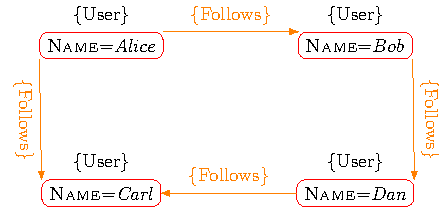
\includegraphics[scale=0.7]{fig/03joins/esn2.pdf}
			\subcaption{ResearchGate graph, Follower relations.}
			\label{g:en}
		\end{minipage}
		\begin{minipage}[b]{0.5\textwidth}
			\centering
			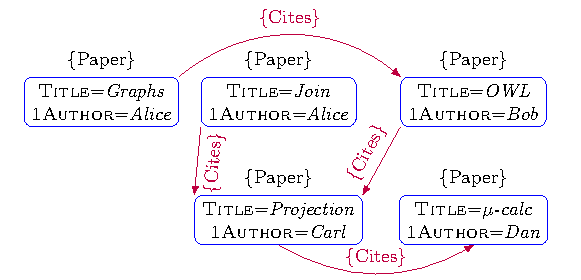
\includegraphics[scale=0.7]{fig/03joins/projects2}
			\subcaption{Reference graph, citation relations. Each paper has a
				first author.}
			\label{g:dep}
		\end{minipage}
	\end{adjustbox}
	\begin{adjustbox}{max width=\textwidth}
		\begin{minipage}[b]{0.5\textwidth}
			\centering
			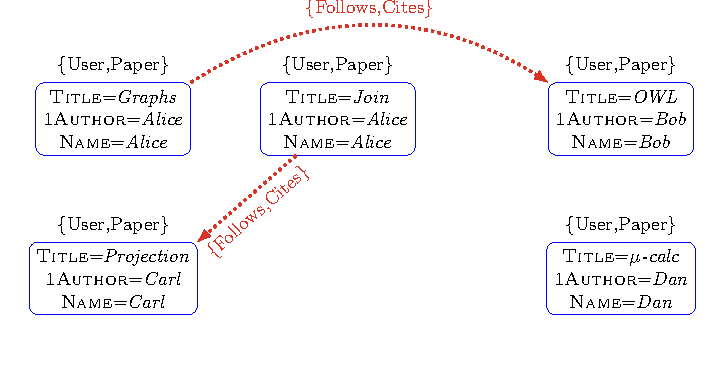
\includegraphics[scale=0.6]{fig/03joins/conj2}
			\subcaption{First query: ResearchGate$\Join^{\wedge}_{\texttt{Name}=\texttt{1Author}}$Reference}
			\label{g:conjo}
		\end{minipage}\quad
		\begin{minipage}[b]{0.5\textwidth}
			\centering
			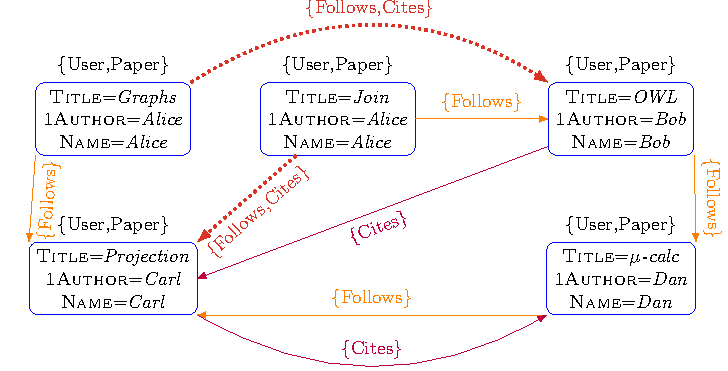
\includegraphics[scale=0.6]{fig/03joins/disj2}
			\subcaption{Second query: ResearchGate$\Join^{\vee}_{\texttt{Name}=\texttt{1Author}}$Reference}
			\label{g:depjo}
		\end{minipage}
	\end{adjustbox}
	\caption{Example of a Graph Database for an Enterprise. Dotted edges remark
		edges  shared between the two different joins.}
	\label{fig:exdb}
\end{figure*}
\begin{figure*}
	\begin{adjustbox}{max width=\textwidth}
		\begin{minipage}[b]{0.5\textwidth}
			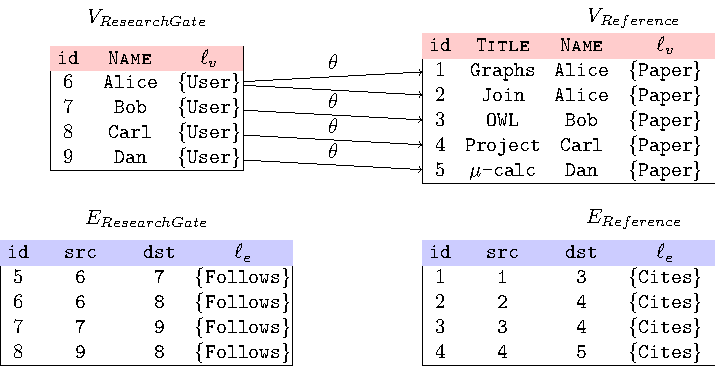
\includegraphics[width=\textwidth]{fig/03joins/reljoins2}
			\subcaption{Representing the operands' vertices and edges with tables. The $\theta$ join
				for the vertices only involves tables $V_{ResearchGate}$ and $V_{projects}$.}
			\label{key}
		\end{minipage}\quad
		\begin{minipage}[b]{0.5\textwidth}
			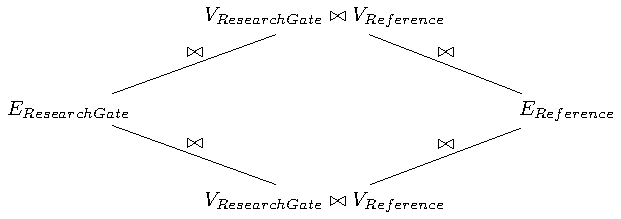
\includegraphics[width=\textwidth]{fig/03joins/queryplan3}
			\subcaption{SQL join query plan required to create edges for ResearchGate$\Join^{\wedge}_{\texttt{Name}=\texttt{1Author}}$Reference. The leaves acts as
				the edges' sources while the root as their destinations.}
			\label{qplan}
		\end{minipage}
	\end{adjustbox}
	\caption{Graphically representing the relational join procedure required to evaluate the first query (Figure \ref{g:conjo}).}
\end{figure*}
As for relational databases, they solve common graph queries efficiently, so GDBMS rely either on relational database engines
\cite{Aberger,Paradies,ErlingM09} or on column store databases \cite{SQLGraph,preSQLGraph}.
Moreover, relational databases already have  efficient implementations for (equi) join algorithms \cite{SchuhCD16}.
We want to show that  graph joins over the relational data model are
not inefficient.
Before all, let us see an example of a graph join query:

\begin{example}\label{ex:one}
	Consider an on-line service such as \textup{ResearchGate} (Figure \ref{g:en}, or Academia.edu)
	where researchers can \textup{follow} each others' work, and a \textup{citation} graph (Figure \ref{g:dep}). Now
	we want to
	``\textit{return the paper graph where a paper cites another one iff.\,\,the \textup{first
			author} \textsc{1Author} of the first paper \textup{follows} the \textsc{1Author} of the second.} (Figure \ref{g:conjo})''. The
	\textup{ResearchGate} graph does not contain any edge regarding the \textup{references}, while the
	\textup{Reference} graph does not contain any information pertaining to the \textit{follow} relations.
	This demands a join between the two graphs: as a first step we
	join the vertices together as in the relational model (vertices are considered
	as tuples using $\textsc{Name}=\textsc{1Auth}$ as a vertex equi-join predicate, $\theta$) and then combine the
	edges from both graphs. Accordingly
	to the query formulation, we establish an edge between two joined vertices
	only if the source has a paper citing the destination, and the
	user in the source follows the user in the destination.
\end{example}
Let us now examine the graph join implementation within the relational model:
vertices and edges are represented as two relational tables (\cite{SQLGraph}, Figure \ref{key}).
In addition to the attributes within the vertices' and the edges' tables,
we assume that each row (on both vertices and edges) has an attribute \texttt{id}
enumerating vertices and edges. Concerning SQL interpretation of such graph join,
we first join the vertices (see the records linked by $\theta$ lines in Figure \ref{key}).
Then the
edges are computed through the join query provided in Figure \ref{qplan}:
the root and the leaves are the result of the $\theta$ join between the vertices,
while the edges appear as the
intermediate nodes. An adjacency list representation of a graph, as the one
proposed in the current paper, reduces the joins within the relation
solution to one (each vertex and edge is traversed only once),
thus reducing the number of required operation to create the resulting
graph.
%Other inefficiency considerations for graph query languages are provided in the Related Work section (Section \ref{sec:pg}).

Example \ref{ex:one} showed only
one possible way to combine the operands' edges, but
we can even return
edges pertaining to both operands as in the following query:
``\textit{For each paper reveal both the direct
	and the indirect dependencies (either there is a direct paper citation,
	or one of the authors follows the other one in ResearchGate)}''.
The resulting graph  (Figure \ref{g:depjo}) has the same vertex set than the previous one, but
they differ on the final edges.
This implies that our graph join definition must be general enough to
allow different edge combinations: we refer to those as
\textbf{edge semantics}, ``\textbf{es}'' for shorthand.

This chapter provides the following main contributions:

\begin{itemize}
	\item \textbf{(binary) Graph $\theta$-join operator}; we first outline a simple graph model in order to
	provide a first intuitive definition of a graph join (see our Technical Report \cite{BergamiMM16} outlined in
	Section \ref{sec:datamodel}). The operator is both commutative (by swapping the graph operands, the result doesn't change) and associative
	(it doesn't matter which graph is joined first).
	Finally, such data model is closed under graph join (i.e. the output of the computation is a graph).
	\item \textbf{\textsc{Graph Conjunctive Equi-join Algorithm} for a specific graph combination task} (``conjunctive'', Section \ref{sec:algo}): we
	compare it to its implementation
	over both graph  (SPARQL, Cypher) and relational (SQL) query languages: as a result our solution outperforms
	the query plan implementation of the other query languages and scales on the large. An example on how to use the same algorithm for less-equal predicate is also prodived (\textbf{\textsc{Graph Conjunctive Less-equal Algorithm}}, Section \ref{sec:lessequaljoin})
  \item Graph Joins are then generalized into \textbf{left}, \textbf{right} and \textbf{full} joins, and it is also showed how to extend the first graph join definition to implement such operators (Section \ref{sec:leftrightfull}). We show how full graph joins can be used to integrate both graph data and graph schemas into one single intermediate representation.
  %\item By extending the concept of binary predicates into edges, Edge Joins are introduced as a preliminary step towards the definition of Graph Nesting (Chapter \vref{cha:nesting}).
\end{itemize}